% generated by experiments/build_paper_assets.py -- do not edit by hand
\begin{figure}[t]
\centering
\resizebox{\linewidth}{!}{%
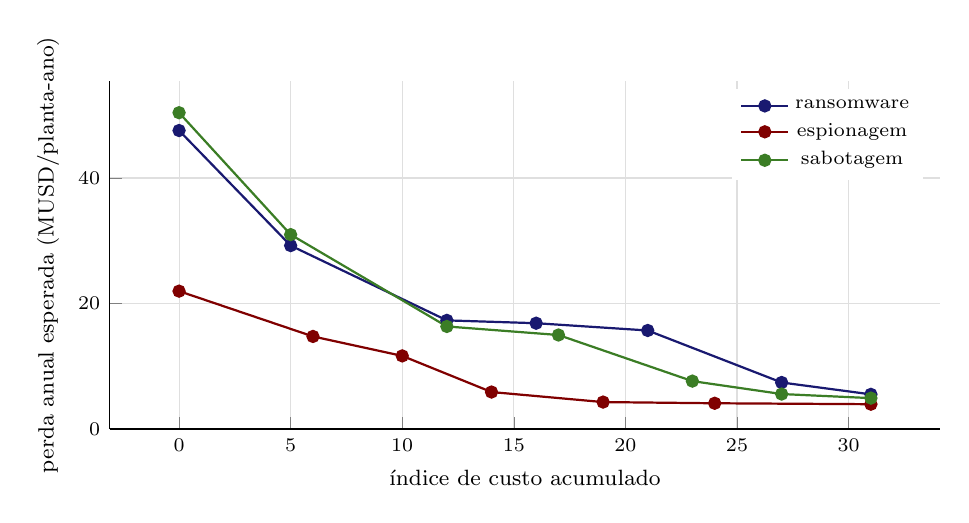
\begin{tikzpicture}
\begin{axis}[
    width=\linewidth, height=6.0cm,
    xlabel={índice de custo acumulado}, ylabel={perda anual esperada (MUSD/planta-ano)},
    ymin=0, legend style={at={(0.98,0.98)}, anchor=north east, font=\scriptsize, draw=none},
    ticklabel style={font=\scriptsize}, label style={font=\footnotesize},
    xmajorgrids, ymajorgrids, grid style={gray!25}, axis lines*=left,
]
\addplot[MidnightBlue, thick, mark=*] coordinates {(0.0,47.57) (5.0,29.23) (12.0,17.31) (16.0,16.86) (21.0,15.7) (27.0,7.41) (31.0,5.52)};
\addplot[Maroon, thick, mark=*] coordinates {(0.0,21.97) (6.0,14.75) (10.0,11.65) (14.0,5.89) (19.0,4.29) (24.0,4.1) (31.0,3.95)};
\addplot[OliveGreen, thick, mark=*] coordinates {(0.0,50.41) (5.0,30.98) (12.0,16.34) (17.0,14.98) (23.0,7.63) (27.0,5.57) (31.0,4.92)};
\legend{ransomware, espionagem, sabotagem}
\end{axis}
\end{tikzpicture}}
\caption{Fronteira eficiente obtida por seleção gulosa sobre a redução marginal de risco por unidade de custo, para cada perfil de ator.}
\label{fig:frontier}
\end{figure}
